\section{Spline-Interpolation}

\begin{minipage}[c]{14.5cm}
Die Idee der Spline-Interpolation ist, die Daten nicht mit einem Polynom hohen Grades zu interpolieren, sondern mit mehreren Polynomen tiefen Grades. Daduch kann die Tendenz  zum Schwingen von Polynomen hohen Grades umgangen werden. Bei den "Bruchstellen", den Übergängen von einem Patch zum nächsten, müssen die Ableitungen der benachbarten Patches bis zu einem vorgegeben Ableitung übereinstimmten.
\end{minipage}
\hfill
\begin{minipage}[c]{4cm}
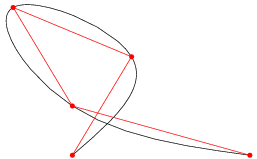
\includegraphics[width=\textwidth]{bilder/kubikSpline}
\end{minipage}

\textbf{Eigenschaften}
\begin{liste}
  \item[\textbf{+}] Kein Runge-Phänomen (Schwingungen am Rand)
  \item[\textbf{+}] Polynome haben tiefen Grad
  \item[\textbf{+}] Aufwand zur Berechnung geringer als Newton [Spline: $O(n)$ (wegen Tridiagonaler Band-Matrix), Newton: $O(n^2)$]  
  \item[$\mathbf{-}$] "`Nicht eingebettet"' (neue Messungen bedeutet, neue Polynomberechnung!)
  \item[$\mathbf{-}$] Polynome müssen zur Auswertung zusammengesetzt werden (Post-Processing Aufwand gross)
\end{liste}


\subsection{Ein-Dimensionale Splines}
\subsubsection{Prinzip}
Pro \em Patch \em (von total $n$) wird ein Polynom vom Grad $d$ (meist kubisch, $d=3$) berechnet. An den Übergängen 
bei $x_i$ können Bedingungen $C^k$ ($k=1,\ldots, d-1$) definiert werden.

\paragraph{Freiheitsgrade}
$n$ Patches mit je 1 Polynom mit je $(d+1)$ Koeffizienten, gibt total $n(d+1)$ Freiheitsgrade.

\paragraph{Bedingungen}
$n$ Patches mit Anfang und Ende $=2n$;
$d-1$ Ableitungen pro innerem Punkt $(n-1)(d-1)$ ergibt total ($(n(d+1)-(d-1))$) Bedingungen.

\paragraph{Zusatzbedingungen}

Vergleicht man Freiheitsgrade und Bedinungen, sind $d-1$ Bedingungen zu wählen. Beim \em natural 
spline \em werden dazu die zweiten Ableitungen auf 0 gesetzt; beim \em clamped splines \em werden
die 1. Ableitungen vorgegeben.


\subsubsection{Allgemeines Vorgehen (kubische Splines)}
Die endgültige Interpolation hat folgende Form (Beschreibung \textbf{eines} Patches):
$$\boxed{S_i(x) = a_i + b_i(x-x_i) + c_i(x-x_i)^2 + d_i(x-x_i)^3}$$
$$S_i' = b_i + 2c_i(x-x_i)+3d_i(x-x_i)^2$$
$$S_i'' = 2c_i + 6 d_i (x-x_i)$$
Gebraucht wird auch (Patch-Breite) $h_i = x_{i+1} - x_i = \Delta x_i$ 
\begin{enumerate}
  \item $a_i = y_i \qquad (i=0,\ldots n-1)$
  \item Für kubische Splines hat es $d-1=3-1=2$ Zusatzbedingungen.\\ 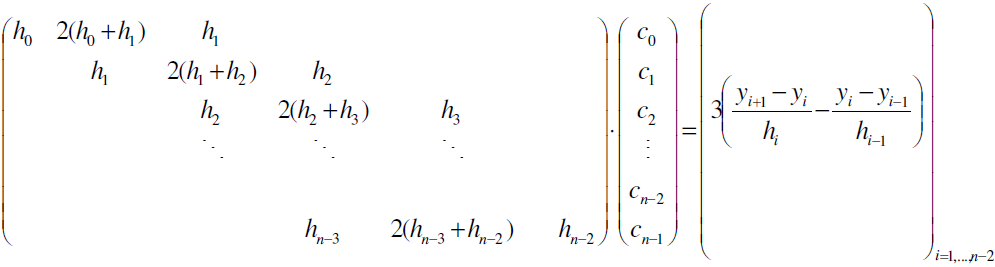
\includegraphics[width=12cm]{./bilder/1d_spline_gleichungssystem}
\newpage
    \begin{itemize}
      \item \textbf{Natural Splining} (Randkrümmung): $y_0''=0=y_n''$ (minimiert das Energiemass! ($\min \int |f''(x)|^2 \mathrm{d}x$))
        \begin{enumerate}
          \item $c_0 = c_n = 0$
          \item Gleichungssystem nach $c_i$ auflösen:\\
            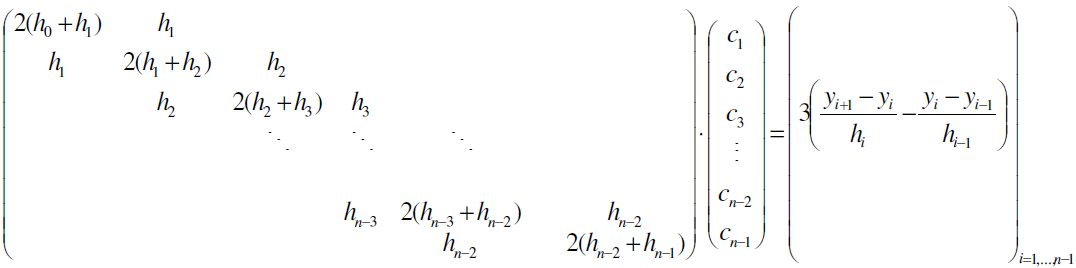
\includegraphics[width=13cm]{./bilder/1d_spline_natural_gleichungssystem}
          %\item $d_{n-1} = -\frac{c_{n-1}}{3h_{n-1}}$
        \end{enumerate}        
       \item \textbf{Clamped Splining:}
         \begin{enumerate}
           \item $b_0 = y_0'; b_n=y_n'$
           \item Gleichungssystem nach $c_i$ auflösen:\\
             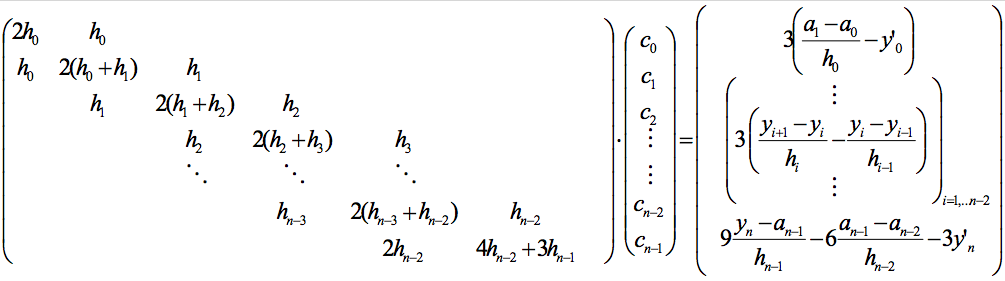
\includegraphics[width=12cm]{./bilder/ClampedSplining}
           %\item $d_{n-1} = \frac{y_n' - b_{n-1} - 2c_{n-1}h_{n-1}}{3h_{n-1}^2}$ (am Schluss zu berechnen)
         \end{enumerate}
    \end{itemize}
  \item $b_{i-1} = \frac{a_i - a_{i-1}}{h_{i-1}} - \frac{2 c_{i-1} + c_i}{3} h_{i-1} \qquad (i=1, \ldots n-1)$
  \item $b_{n-1} = \frac{y_n - a_{n-1}}{h_{n-1}} - c_{n-1} h_{n-1} - d_{n-1}h_{n-1}^2=\frac{y_n-y_{n-1}}{h_{n-1}}-\frac 23 c_{n-1}h_{n-1}$
  \item $d_{i-1} = \frac{c_i - c_{i-1}}{3 h_{i-1}} \qquad (i=1, \ldots n-1)$
  \item Clamped splining: $d_{n-1} = \frac{y_n' - b_{n-1} - 2c_{n-1}h_{n-1}}{3h_{n-1}^2}$ \hspace{1cm} Natural Splining: $d_{n-1} = -\frac{c_{n-1}}{3h_{n-1}}$
\end{enumerate}

\paragraph{Weitere Methoden}~\\
Bei \emph{Hermite cubic splines} werden $C^1$-Funktionen aus gepatchten kubischen Polynomen mit
vorgegebenen ersten Ableitungen gebildet.

\emph{Periodic splines} sind $C^2$ Funktionen aus gepatchten kubischen Polynomen mit Periodizität ($S'(x_0)=S'(x_n)$ und $S''(x_0)=S''(x_n)$).

\subsubsection{Fehlerabschätzung}
Für kubische Splines mit $C^2$ gilt folgende Fehlerabschätzung ($H = \max h_i \; (i=0, \ldots n-1)$):\\
$| y(x) - S(x) | \leq \max |y^{(4)}(x)| \frac{5}{384} H^4 \qquad
 | y'(x) - S'(x) | \leq \max |y^{(4)}(x)| \frac{1}{24} H^3 \qquad 
 | y''(x) - S''(x) | \leq \max |y^{(4)}(x)| \frac{3}{8} H^2$
 
 
\newpage
\subsection{Bernstein-Bézier Splines (B-B Splines)}

\begin{minipage}[c]{15.0cm}	
	\subsubsection{Bernstein-Polynome}
    	Die Bernstein-Polynome sind im Intervall $t\in[0,1]$ definiert als
	    \[B_{i,n}(t) = \binom{n}{i}(1-t)^{n-i} t^i \qquad t \in [0,1]\; i=0,1,\ldots, n\]
	    mit $i$: Nr und  $n$: Ordnung des Splines.
	    
        Mittels einer affinen Transformation in den Bereich $t \in [a,b]$ folgt	    
	    \[B_{i,n}(u,a,b) =\frac{1}{(b-a)^n}\binom{n}{i}(b-u)^{n-i} (u-a)^i \qquad u \in [a,b]\; i=0,1,\ldots, n\]
	    
	\paragraph{Eigenschaften}
		Bernstein Polynome$\ldots$
	    \begin{itemize}
	      \item ergeben eine lineare Basis für Polynome der Ordnung $n$ (man kann mit ihnen jedes Polynom der Ordnung $n$ zusammenbauen)
	      \item haben genau eine Maximalstelle bei $t=\frac in$
	      \item haben eine Nullstelle bei $0$ (Ordnung $i$) und bei $1$ (Ordnung $n-1$)
	      \item sind symmetrisch: $B_{i,n}(t) = B_{n-i,n}(1-t)$
	      \item sind zwischen $t \in [0,1]$ begrenzt auf $[0,1]$
	      \item ergeben in der Summe: $\sum \limits_{i=0}^n B_{i,n}(t)=1$
	    \end{itemize}
	    
	    $\frac{d}{dt} B_{i,n}(t) = n(B_{i-1,n-1}(t) - B_{i,n-1}(t)) = -n \Delta B_{i-1,n-1}(t)$\\
	    $\frac{d^2}{dt^2} B_{i,n}(t) = n(n-1)(B_{i-2,n-2}(t) -2 B_{i-1,n-2}(t) + B_{i,n-2}(t)) = n(n-1) \Delta^2 B_{i-2,n-2}(t)$\\
	    $\frac{d^k}{dt^k} B_{i,n}(t) = (-1)^k n(n-1)\ldots(n-k+1) \Delta^k B_{i-k,n-k}(t)$
\end{minipage}
\hfill    
\begin{minipage}[c]{4cm}
  	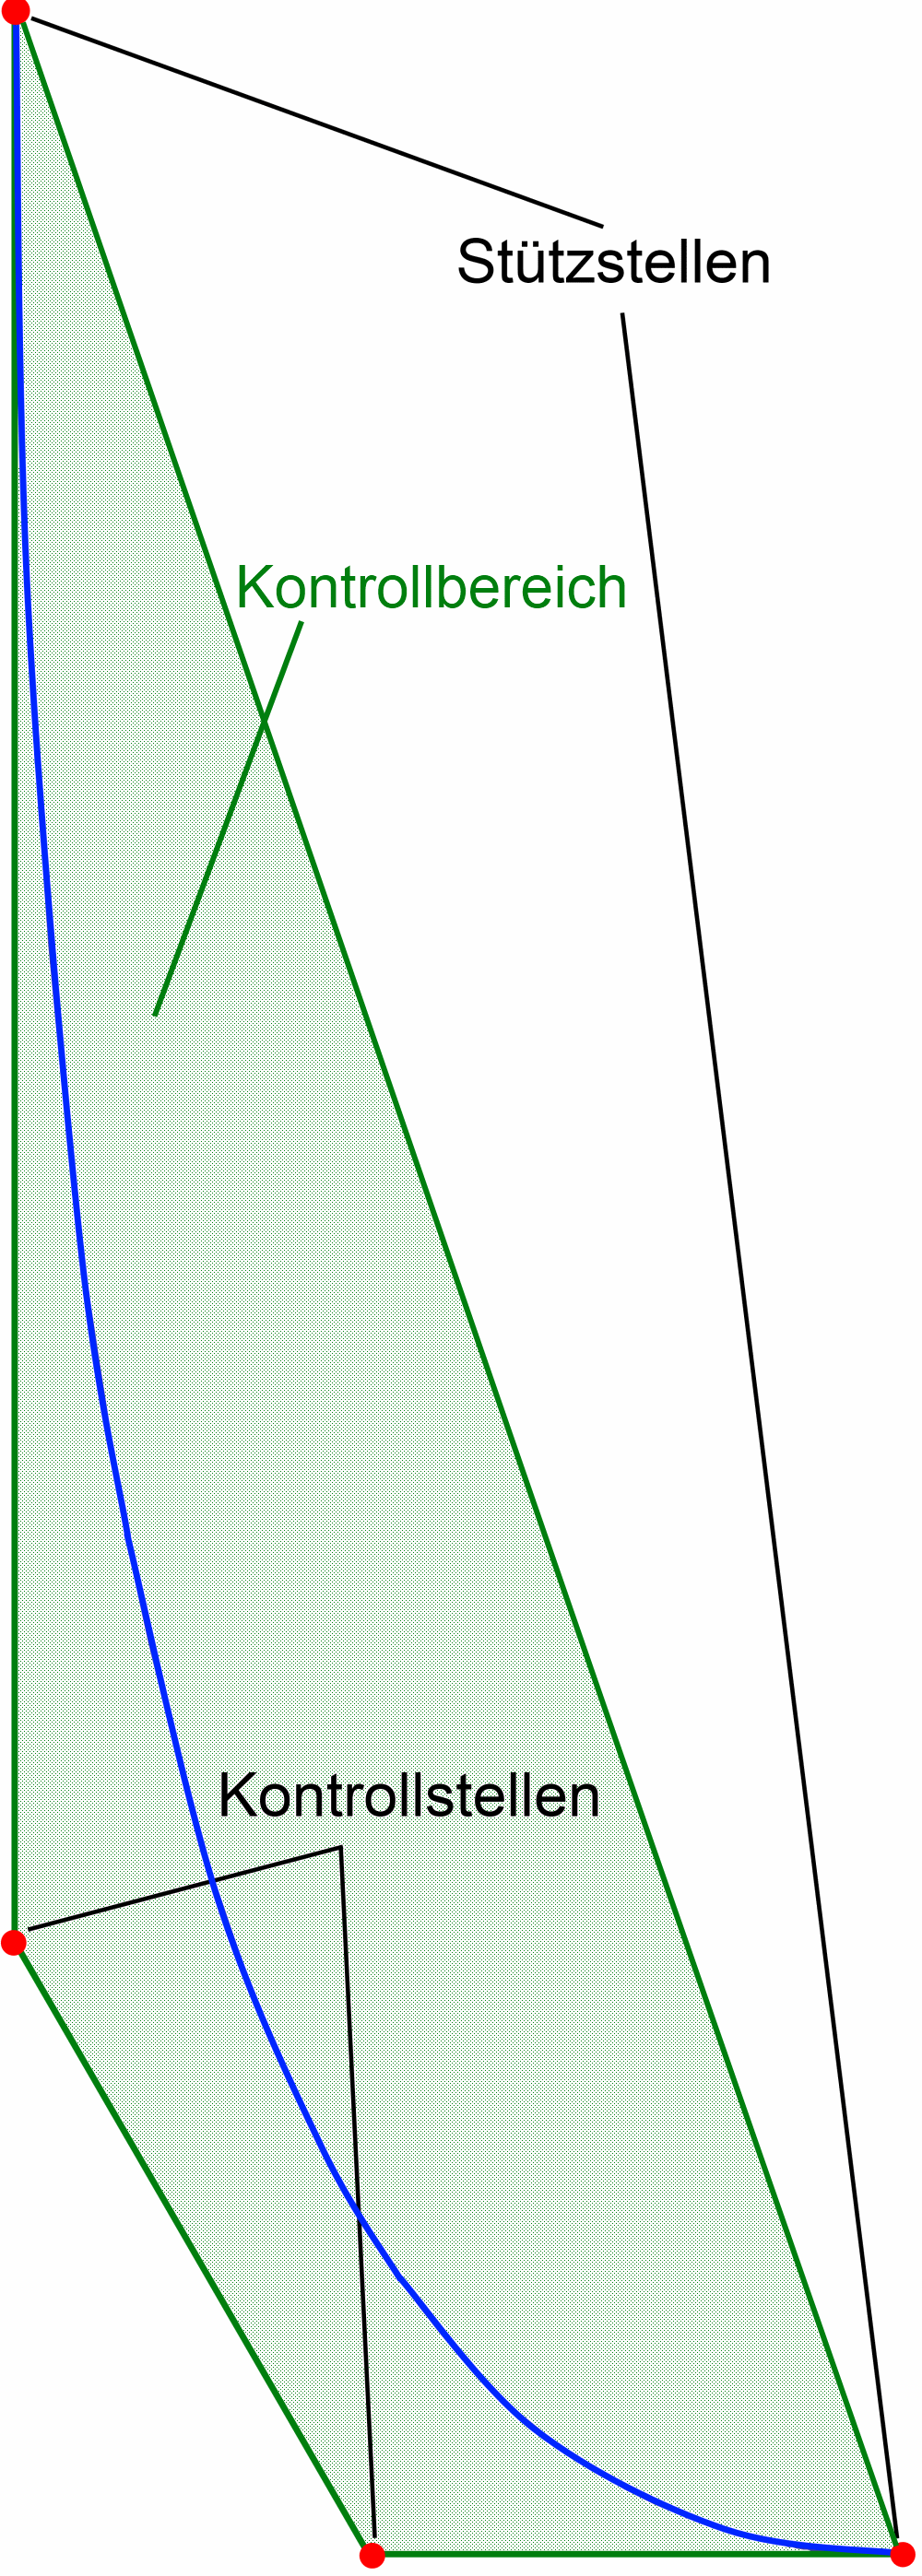
\includegraphics[width=\textwidth]{bilder/bernsteinBezier}
\end{minipage}

\vspace{0.2cm}

\begin{minipage}[c]{5.5cm}	
\textbf{Pascal'sches Dreieck}\\

	\scalebox{0.8}{
	\renewcommand{\arraystretch}{1}
	\begin{tabular}{rccccccccc}
		$n=0$:&    &    &    &    &  1\\\noalign{\smallskip\smallskip}
		$n=1$:&    &    &    &  1 &    &  1\\\noalign{\smallskip\smallskip}
		$n=2$:&    &    &  1 &    &  2 &    &  1\\\noalign{\smallskip\smallskip}
		$n=3$:&    &  1 &    &  3 &    &  3 &    &  1\\\noalign{\smallskip\smallskip}
		$n=4$:&  1 &    &  4 &    &  6 &    &  4 &    &  1\\\noalign{\smallskip\smallskip}
	\end{tabular}}
\end{minipage}
\hfill    
\begin{minipage}[c]{13.25cm}   
\textbf{Bernstein Polynome} \quad $0\leq t\leq 1$\\

	\scalebox{0.8}{
	\begin{tabular}{lllll}
		$B_{0,0}(t)=1$&&&&\\
		$B_{0,1}(t)=1-t$&$B_{1,1}(t)=t$&&&\\
		$B_{0,2}(t)=(1-t)^2$&$B_{1,2}(t)=2t(1-t)$&$B_{2,2}(t)=t^2$&&\\
		$B_{0,3}(t)=(1-t)^3$&$B_{1,3}(t)=3t(1-t)^2$&$B_{2,3}(t)=3t^2(1-t)$&$B_{3,3}(t)=t^3$&\\
		$B_{0,4}(t)=(1-t)^4$&$B_{1,4}(t)=4t(1-t)^3$&$B_{2,4}(t)=6t^2(1-t)^2$&$B_{3,4}(t)=4t^3(1-t)$&$B_{4,4}(t)=t^4$\\
	\end{tabular}}
\renewcommand{\arraystretch}{1.5} 
\end{minipage}  


\subsubsection{Simple Bézier Kurven}
Eine Bézier-Kurve wird über Kontrollpunkte ($\vec{P}_0, \vec{P}_1, \ldots \vec{P}_n\,(n \geq 2)$ 
in $R^d$) sowie die Bernstein Polynome definiert:
$$\vec{r}(t) = \sum \limits_{i=0}^{n} \vec{P}_i B_{i,n}(t) \quad t \in [0,1]$$
\paragraph{Eigenschaften}
\begin{itemize}
  \item Die Bézier-Kurven liegen immer innerhalb der konvexen Hülle der Kontrollpunkte.
  \item \begin{tabular}{ll}
            $\vec{r}(0) = \vec{P}_0$ & $\vec{r}(1) = \vec{P}_n$ \\
            $\vec{r}\,'(0) = n(\vec{P}_1-\vec{P}_0)$ & $\vec{r}\,'(1) = n(\vec{P}_n-\vec{P}_{n-1})$ \\
            $\vec{r}\,''(0) = n(n-1)(\vec{P}_2 - 2\vec{P}_1 + \vec{P}_0)$ & $\vec{r}\,''(1) = n(n-1)(\vec{P}_n - 2\vec{P}_{n-1} + \vec{P}_{n-2})$ \\
        \end{tabular}
  \item Wenn $C^k$ Übergang zu einem Punkt gefordert ist, sind $k$ Gleichungen bzw. $k$ 
        Kontrollpunkte pro Punkt nötig
\end{itemize}

\begin{minipage}{13.5cm}
\subsubsection{Casteljau recurrence}
Die Castaljau recurrence ist eine ähnliche Idee wie Neville-Aitken. 
Damit kann ein Punkt auf einer Bézier Kurve als Linearkombination zweier Punkte aus Bézier Kurven tieferer Ordnung berechnet werden.
\[
    \vec{r}_{\vec{P_0},\vec{P_1},\ldots,\vec{P_n}}(t) = (1-t)\cdot\vec{r}_{\vec{P_0},\vec{P_1},\ldots,\vec{P_{n-1}}}(t) + t \cdot \vec{r}_{\vec{P_1},\vec{P_2},\ldots,\vec{P_n}}(t) \qquad t \in [0,1]
\]


  \subsubsection{Zusammengesetzte (Composite) Bézier Kurven}
  Die zusammengesetzten (simplen) Bézier-Kurven sollen die bekannte Bedingungen ($C^k$) erfüllen.
  Dies sind die Gleichungen um den Punkt $Q_0$ mit Kontrollpunkten $Q_{1,\ldots,m-1}$ nach $Q_0$ sowie
  den Kontrollpunkten $P_{1,\ldots,n-1}$ vor $Q_0$. 
\end{minipage}
\begin{minipage}{5.5cm}
  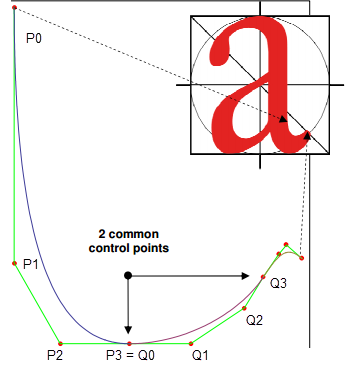
\includegraphics[width=5.5cm]{./bilder/composite_bezier.png}
  Hier sind $m=n=3$
\end{minipage}

  \begin{align*}
      &C^0: \qquad && &&\boxed{\vec{P_n} = \vec{Q_0}} \\
      &C^1: && \vec{r}\,'_P(1) = &&\boxed{n(\vec{P}_n-\vec{P}_{n-1}) = m(\vec{Q}_1-\vec{Q_0})} && = \vec{r}\,'_Q(0) \\
      &C^2: && \vec{r}\,''_P(1) = &&\boxed{n(n-1)(\vec{P}_n - 2\vec{P}_{n-1} + \vec{P}_{n-2}) = 
    m(m-1)(\vec{Q}_2 - 2\vec{Q_1} + \vec{Q_0})} && = \vec{r}\,''_Q(0) \\
      &C^k: && \vec{r}_P^{\,(k)}(1) = && \boxed{n(n-1)\dots(n-k+1)(\Delta^k\vec{P}_{n-k}) = 
      m(m-1)\dots(m-k+1)(\Delta^k\vec{Q}_0)} &&= \vec{r}_Q^{\,(k)}(0)
  \end{align*}
  
  $m$ ist dabei der Grad von $\vec{r}_Q$, $n$ derjenige von $\vec{r}_P$.

\subsubsection{Zusammengesetzte (Composite) Bézier Kurven mit $P_{i,j}$}
  Wird $\vec{r_j}(t) = \sum \limits_{i=0}^{n} \vec{P}_{i,j} B_{i,n}(t) \quad t \in [0,1]$ mit den Fixpunkten $Q_j$ definiert (Grad: $n$), ergeben sich folgende Formeln:

  \begin{align*}
      &C^0: \qquad && &&\boxed{\vec{P}_{n,j-1} = \vec{P_{0,j}} = \vec{Q_j}} \\
      &C^1: && \vec{r}\,'_{j-1}(1) = &&\boxed{\vec{Q}_{j}-\vec{P}_{{n-1,j-1}} = \vec{P}_{1,j}-\vec{Q}_j} && = \vec{r}\,'_j(0) \\
      &C^2: && \vec{r}\,''_{j-1}(1) = &&\boxed{\vec{Q}_{j} - 2\vec{P}_{n-1,j-1} + \vec{P}_{n-2,j-1} = 
    \vec{P}_{2,j} - 2\vec{P}_{1,j} + \vec{Q_j}} && = \vec{r}\,''_j(0) \\
      &C^k: && \vec{r}_{j-1}^{\,(k)}(1) = && \boxed{\Delta^k\vec{P}_{n-k,j-1} = \Delta^k\vec{P}_{0,j}} &&= \vec{r}_j^{\,(k)}(0)
  \end{align*}
  
\subsubsection{Bézier Oberflächen als Tensor Splines}
Bézier Oberflächen werden gleich wie Bézier Kurven mittels einem Tensorprodukt aus Bernstein Polynomen gebildet.
Eine Oberfläche im Intervall $[0,1]\times[0,1]$ wird gebildet durch
\[
    \vec{z}(s,t) = \sum\limits_{i=0}^n\sum\limits_{j=0}^m \vec{P}_{ij} B_{in}(s) B_{jm}(t) \qquad s,t\in[0,1]
\]

Details und Formeln siehe Skript S. 19 -- 23.

\subsubsection{Vergleich Bézier- und Newton-Interpolation mit gleichverteilten Argumenten auf X-Achse}
  Aus Sicht Bézier:
  \begin{liste}
    \item[+] Kleiner Fehler, keine Oszillation, kein Runge (bei kleinem Grad, z.B. 3)
    \item[+] $O(n)$ (linearer Rechenaufwand)
    \item[-] Nicht eingebettet (neue Daten brauchen Neuberechnung der Interpolation)
    \item[-] Post-Processing (Grafik, Integrations, Ableitungen) sind komplexer, da jedes Kurvenstück
      einzeln betrachtet werden muss.
  \end{liste}
